

\chapter{Discussion and Future Work}
\label{Discussion}

\section{Introduction}
\label{Discussion:Intro}

\section{Participatory approaches}
\label{Discussion:RQ1}
\begin{quote}
\textbf{    Research Question 1:
}    
\textit{    “How can we use participatory design approaches to provide meaningful and engaging experiences for people with dementia?”}
\end{quote}

Throughout the thesis, I addressed participatory design approaches in various ways. Chapter four examined a series of participatory design approaches to engage with people with dementia and their families. Through working closely with the families, I adapted traditional participatory methods to fit the needs of the participants, such as creating family days out in which participants would take part in walking interviews. Following on from this work, I was motivated to explore how to broaden these participatory methods to function within the context of larger-scale community events seen in chapter five - that prompted me to explore how hackathons could provide a creative and inclusive space for the public to engage the topic of dementia. 

However, while I gained reasonable interest from designers, developers and students, the event significantly under-represented people with dementia and their care partners. The failure to represent and involve people with dementia in public engagement had multiple knock-on effects on teams' outputs. Still, it provided an opportunity to reflect on the appropriateness of hackathon structures for people with dementia and propose alternatives for collaborative design events. Finally, in chapter seven, I worked with people with dementia, designers, and developers to understand how these different stakeholders may collaborate in building technology. With this in mind, two considerations that arise in responding to the research question are: a) designing for contested realities and b) how we design for research to practice.

\section{Ethical implications in Dementia and HCI}
\label{Discussion:RQ2}
\begin{quote}
\textbf{    Research Question 2:
}    
\textit{    “What are the ethical implications for people with dementia to participate in HCI research?”}
\end{quote}
Across all the studies in this thesis, there has been ongoing ethical implications in how we involve and perceive people with dementia in HCI research. In particular, chapters four and six delve into such challenges in several ways. For chapter four,  I describe initial insights into my understandings of representation within dementia that encompasses my time at Silverline Memories and reflections on family history of dementia. As I explained at the end of chapter four discussion, the critical area that I felt remained underexamined was the ethical implications apparent in our work as a community of practice. This led to chapter six, where I invited 22 HCI and dementia researchers to reflect on their everyday experiences of working with people with dementia and the complexities that may arise in technology or institutional ethics. Through this thesis, exploring these ethical challenges led to more profound insights into the ways we represent and acknowledge people with dementia, and exploration into the 'ruling relations' that shape people with dementia's experiences. 

\section{Supporting meaningful dialogue}
\label{Discussion:RQ3}
\begin{quote}
\textbf{    Research Question 3:
}    
\textit{    “How can we support meaningful dialogue between the public, designers, developers, and people with dementia?”}
\end{quote}
In my literature review on the representation of dementia in the public eye, it is common for people with dementia to be stigmatised surrounding their abilities to communicate and socialise with others. As discussed in chapter four, I adapted the interview approaches to suit the family's needs by co-design days out, which supported meaningful dialogue between myself and the families with dementia. However, on a more comprehensive approach to this research question, chapter five - DemVR, and chapter seven - designing a collaborative toolkit, directly considers ways to facilitate an engaging and meaningful dialogue between the public, designers, developers, and people with dementia. In both chapters, I facilitated conversations surrounding ways technology can promote dialogue between the public and people with dementia. Chapter five deployed an online platform - Ideaboard, where designers, developers, people with dementia and care partners could take part in short consultations to share ideas for VR experiences to be explored in the hackathon. As I report in the chapter, this was a disfavoured platform that was lacked the engagement I had hoped for. In the discussion, I highlight issues of participant disinterest and how the platform was not intentionally built with people with dementia in mind. 

For the final data chapter, I build upon these mistakes to consider what toolkits and technologies could we use to support dialogue between people with dementia and technologists. In conducting this work with designers, developers and people with dementia from the ground-up, the findings demonstrated two priorities for making meaningful dialogue between the different communities - acknowledgement in contribution and how individuals may want to engage with one another.

\section{Competing interests}
\label{Discussion:RQ4}
\begin{quote}
\textbf{    Research Question 4:
}    
\textit{    “What are the competing interests and expectations for dementia design research when involving multiple stakeholders - such as people with dementia, developers, designers and researchers?”}
\end{quote}
From the breadth of literature in HCI and dementia, there is a clear indication towards tailoring technology and design approaches to the needs and desires of people with dementia and their family [cite]. Additionally, throughout the entire thesis, I have explored the competing interests of several stakeholders who impact technology development, such as designers, developers and researchers. By broadening the public conversation around dementia and HCI, the thesis contributes a series of insights into ways we may support conversations between technologists and people with dementia; ways to design for designer and developer workflows; and the challenges in designing for when the reality of the person with dementia is contested. With this in mind, this final section regarding the research questions will discuss a) ways we might design for contested realities and b) constructing a 'we' community between multiple communities. 

\subsection{Designing for contested realities}
\label{RQ4:ContestedRealities}

\section{Future work}
\label{FutureWork}

\subsection{Future studies}
\label{FutureStudies}
The following section builds on the four data chapters to move beyond the abstract discussions found in the previous data chapters to present four exciting studies for future work within technology and dementia. Through these prospective studies, I have attempted to articulate what the abstract directions I have suggested may entail acting as inspiration for researchers who wish to build onto this work. In each future study, I propose a research question with a clear explanation of how this ties into prior work found in this thesis and why it is important for the future of dementia and HCI.

\subsubsection{Ageing in a virtual world}
\label{FutureStudyOne}

\begin{figure}[htp]
\centering
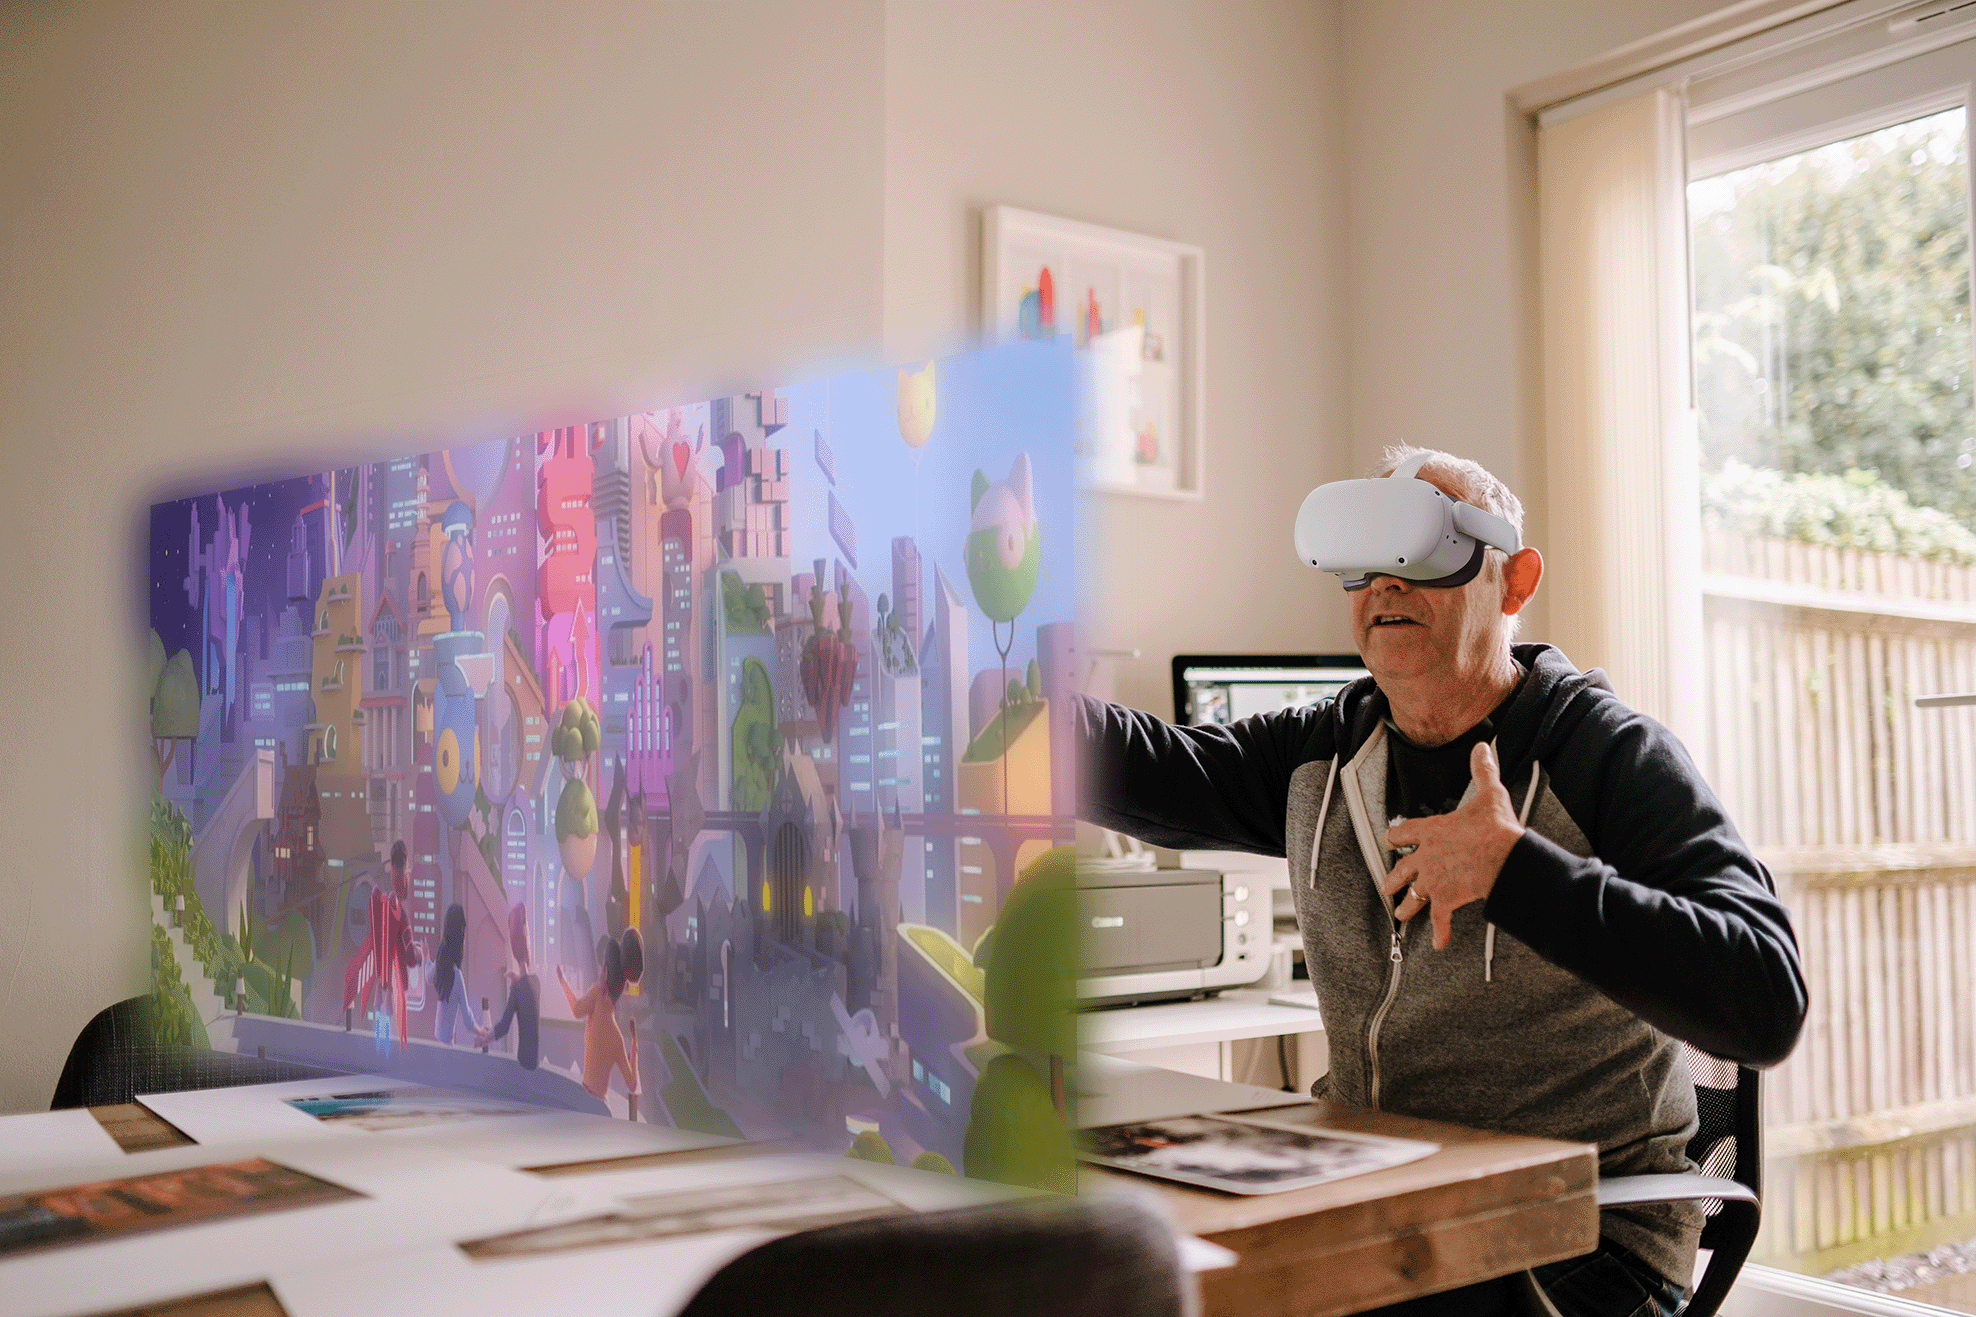
\includegraphics[width=1\linewidth]{Images/Discussion/Aging_in_VR.png}
\caption{Older adult exploring VR spaces}
\label{fig:Aging_VR}
\end{figure}

\subsubsection{Design with Inclusion}
\label{FutureStudyTwo}

\begin{figure}[htp]
\centering
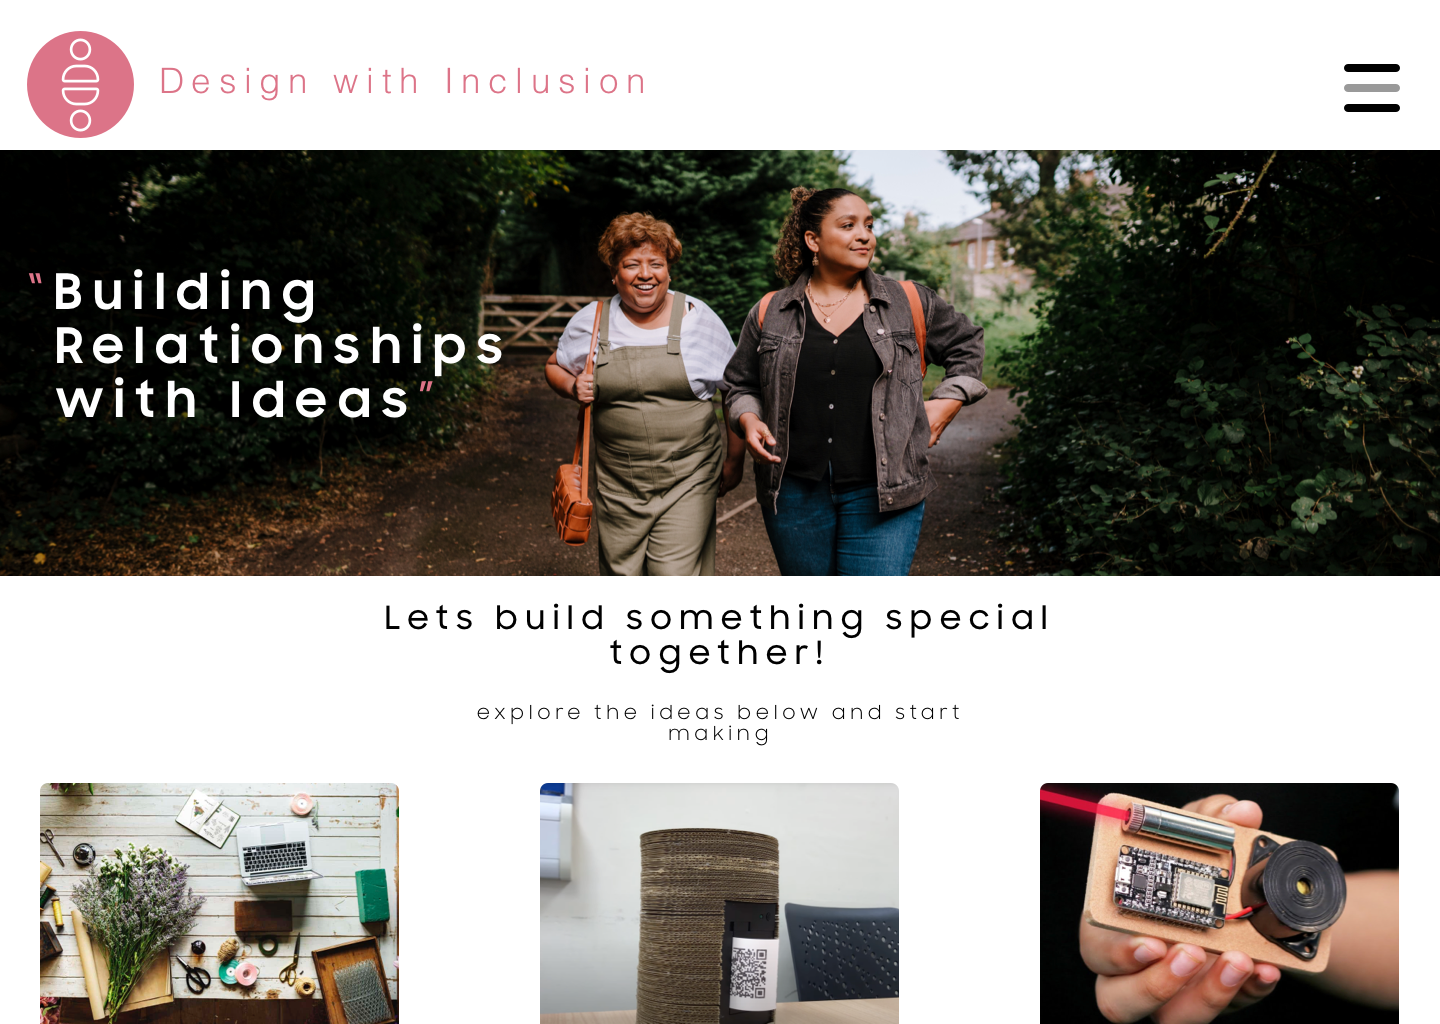
\includegraphics[width=1\linewidth]{Images/Discussion/Design_For_Inclusion.png}
\caption{Design with Inclusion website mockup}
\label{fig:DesignInclusion}
\end{figure}

\subsubsection{Aware-AI}
\label{FutureStudyThree}
\begin{figure}[htp]
\centering
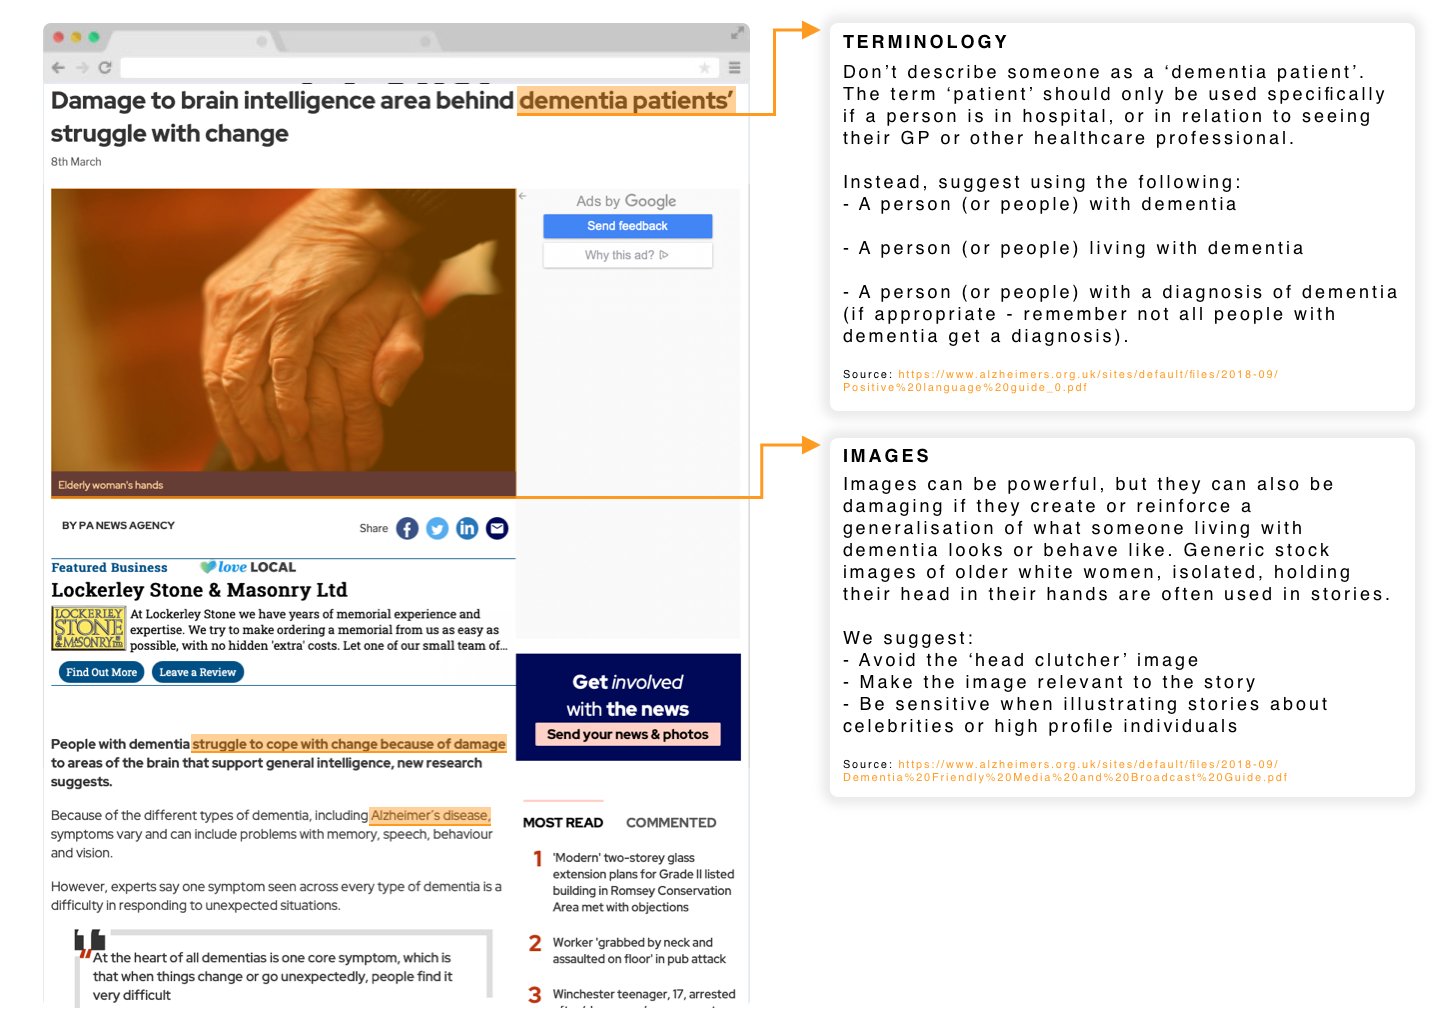
\includegraphics[width=1\linewidth]{Images/Discussion/Aware-AI.png}
\caption{Mockup of Aware-AI in action}
\label{fig:AwareAI}
\end{figure}

\subsubsection{Nothing about us, without us}
\label{FutureStudyFour}

\begin{figure}[htp]
\centering
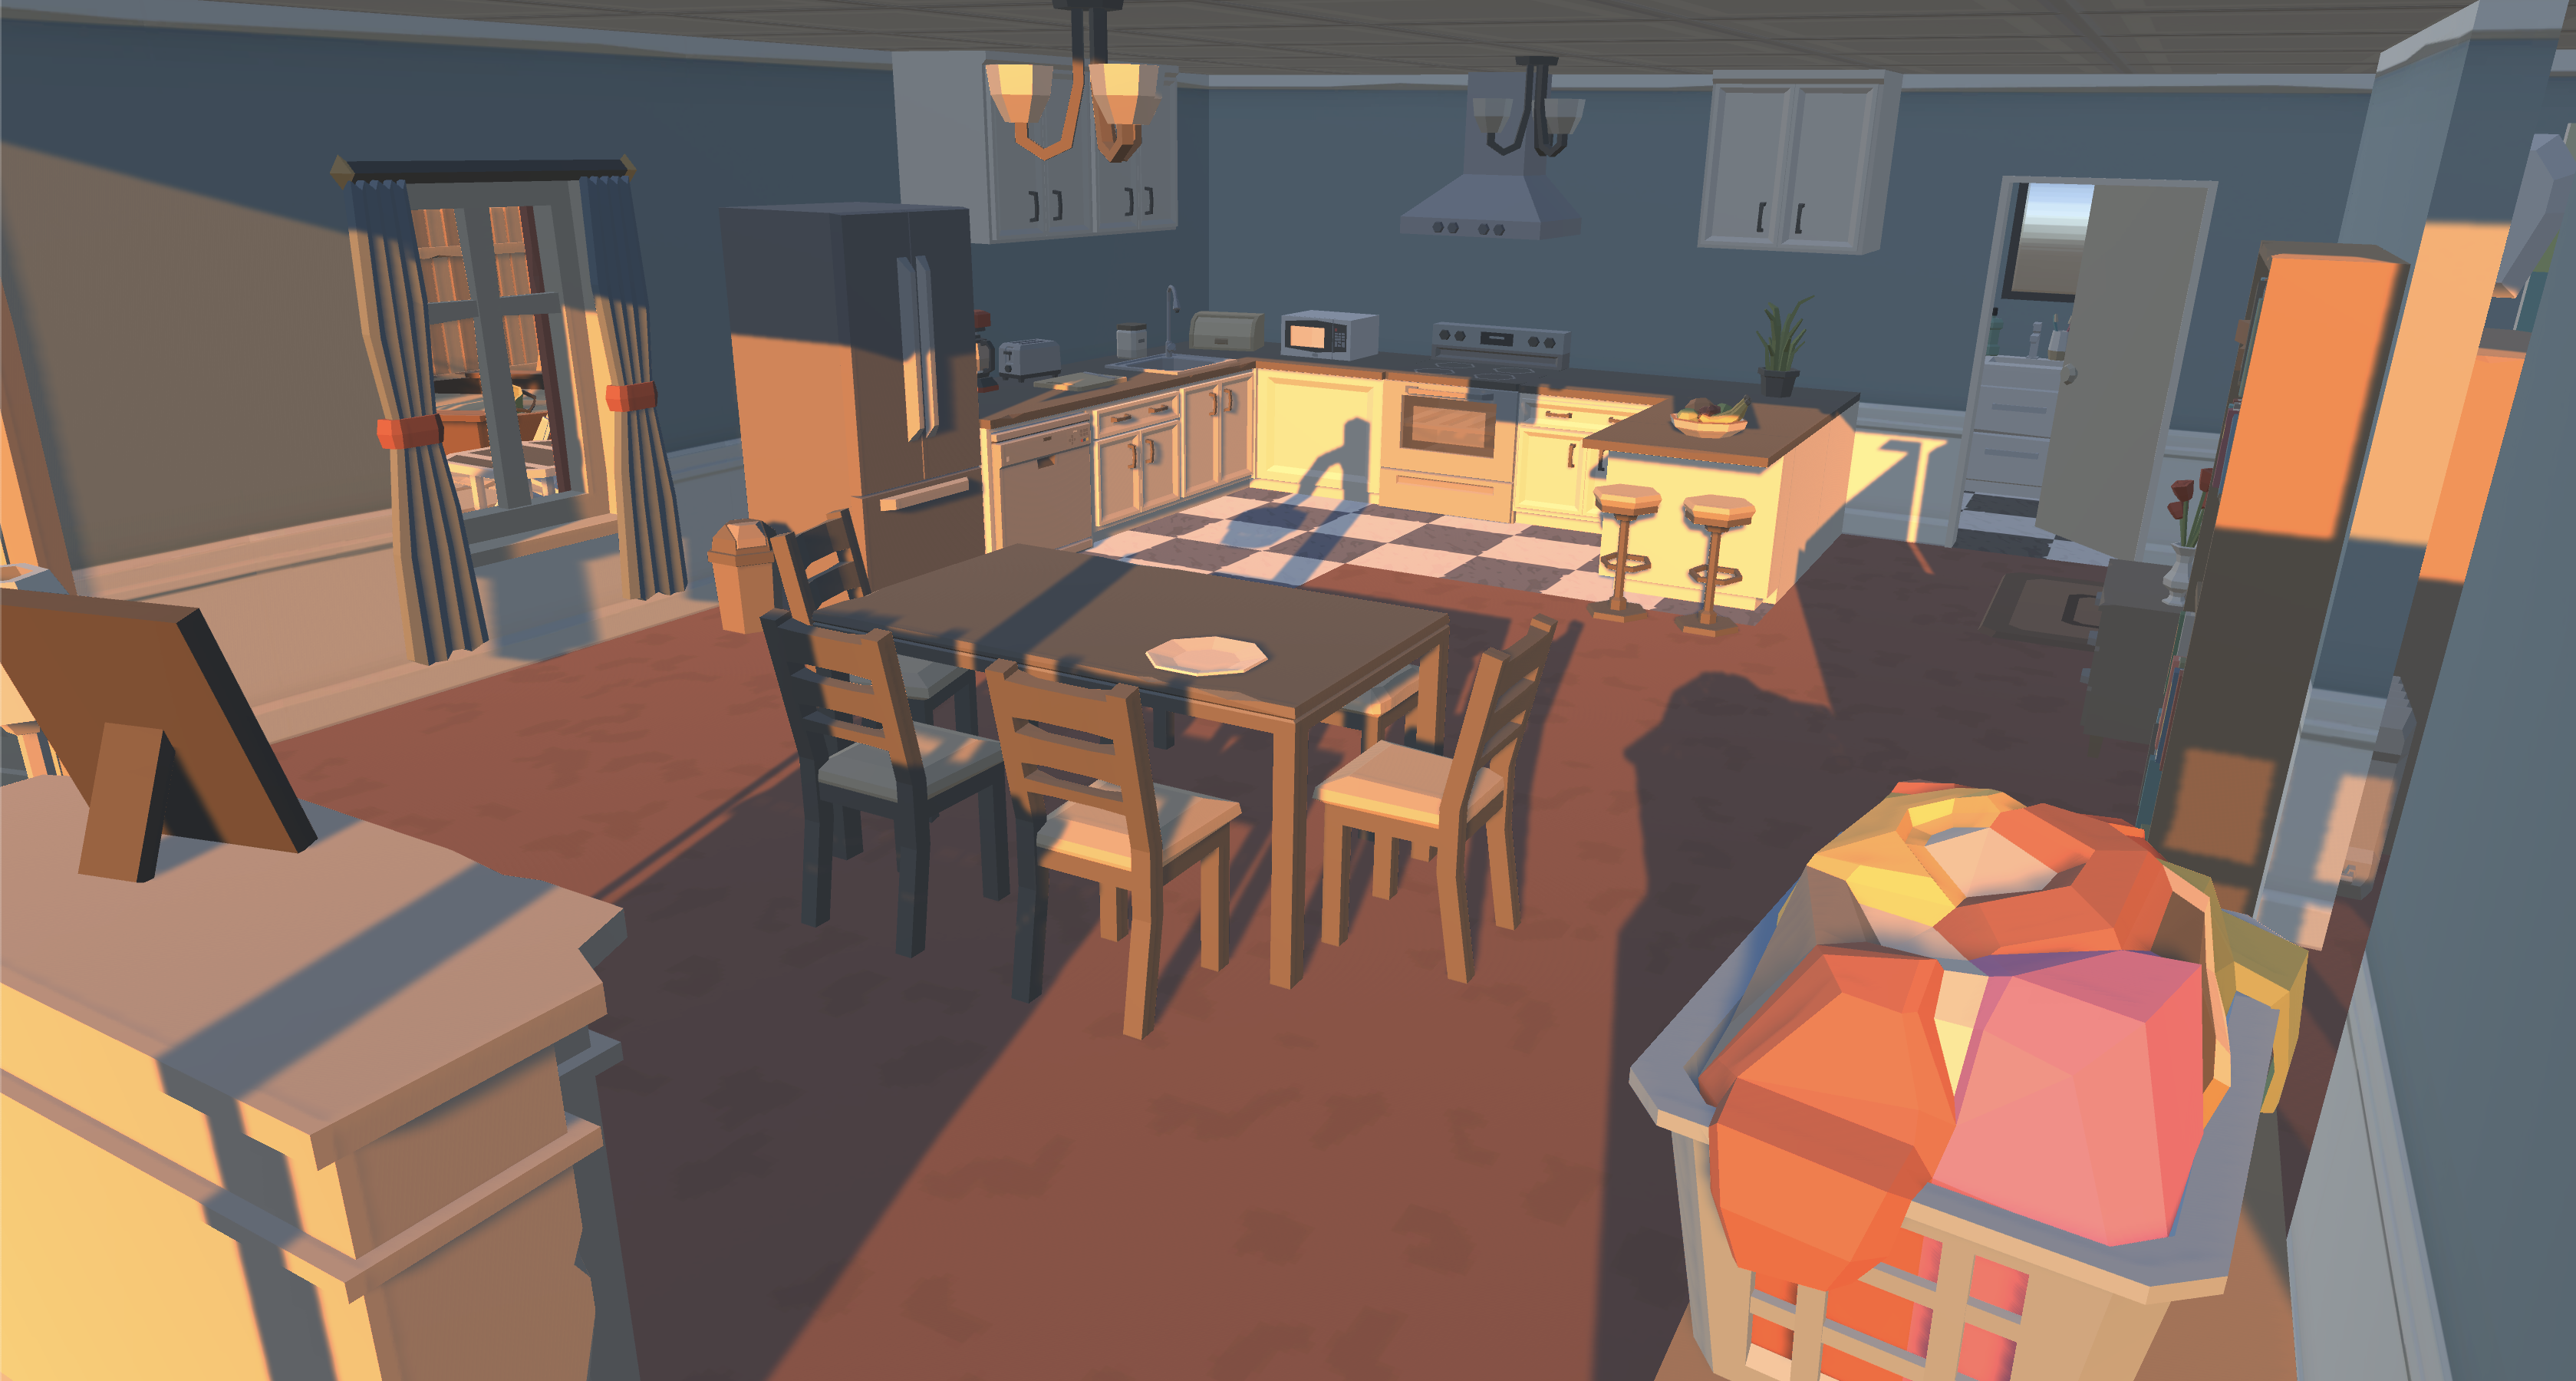
\includegraphics[width=1\linewidth]{Images/Discussion/Storytellling_Game.png}
\caption{Low-poly styling of a home for the game where the player can explore the person with dementia's story and learn about representation and stigma}
\label{fig:StorytellingLowPoly}
\end{figure}

\subsection{Final remarks}
\label{Discussion:FinalRemarks}